% ======= LaTeX Setup ======= %
\documentclass[11pt]{article}
\usepackage[letterpaper, margin=1in]{geometry}
\usepackage{times}
\usepackage{indentfirst}
\usepackage{booktabs}
\usepackage{tabularx}
\usepackage{float}
\usepackage{amsmath}
\usepackage{amssymb}
\usepackage{graphicx}
\newcolumntype{L}{>{\raggedright\arraybackslash}X}
\linespread{1.15}
\setcounter{tocdepth}{2}
\usepackage[hidelinks]{hyperref}
\usepackage{caption}
\captionsetup{font=small, labelfont=bf}

\title{{\large ES100 Project Proposal}\\[0.5em]
On-Device Classification of Neural Action Potentials\\
for Wireless Unit Transmission over Bluetooth Low Energy}
\author{Fredrik Willumsen Haug \\[0.3em]
{\normalsize Bioengineering} \\[0.6em]
{\normalsize Advised by Dr.\ Saehyuck Oh and Professor Gage Hills}}
\date{}

\begin{document}

\maketitle
\thispagestyle{empty}
\clearpage
\setcounter{page}{1}

\tableofcontents
\clearpage

% ======= 0. Executive Summary ======= %
\setcounter{section}{-1}
\section{Executive Summary}
This thesis proposal addresses a bandwidth bottleneck in wireless neural recording. Bluetooth
Low Energy 6.0 (BLE), the leading low-power off-the-shelf wireless communication protocol, has a theoretical
data rate ceiling of 2~Mbps. Neural action potentials, also called spikes, contain frequencies
from 300~Hz to 6~kHz. Raw extracellular neural electrophysiology data is therefore sampled at 30~kHz
to preserve signal integrity for offline identification of individual
neurons appearing on overlapping recording channels. With a 16-bit resolution, each channel generates 480~kbps, imposing a
theoretical four-channel recording ceiling for wireless transmission. Modern high-density recording
probes, however, carry up to thousands of channels, so transmitting their entire raw data over BLE is
currently impossible. The proposed project instead performs neural identification on-device, yielding an
off-the-shelf solution for wireless transmission of putatively identified neurons
compatible with modern rodent neural recording systems.

\vspace*{\fill}

\begin{figure}[H]
\centering
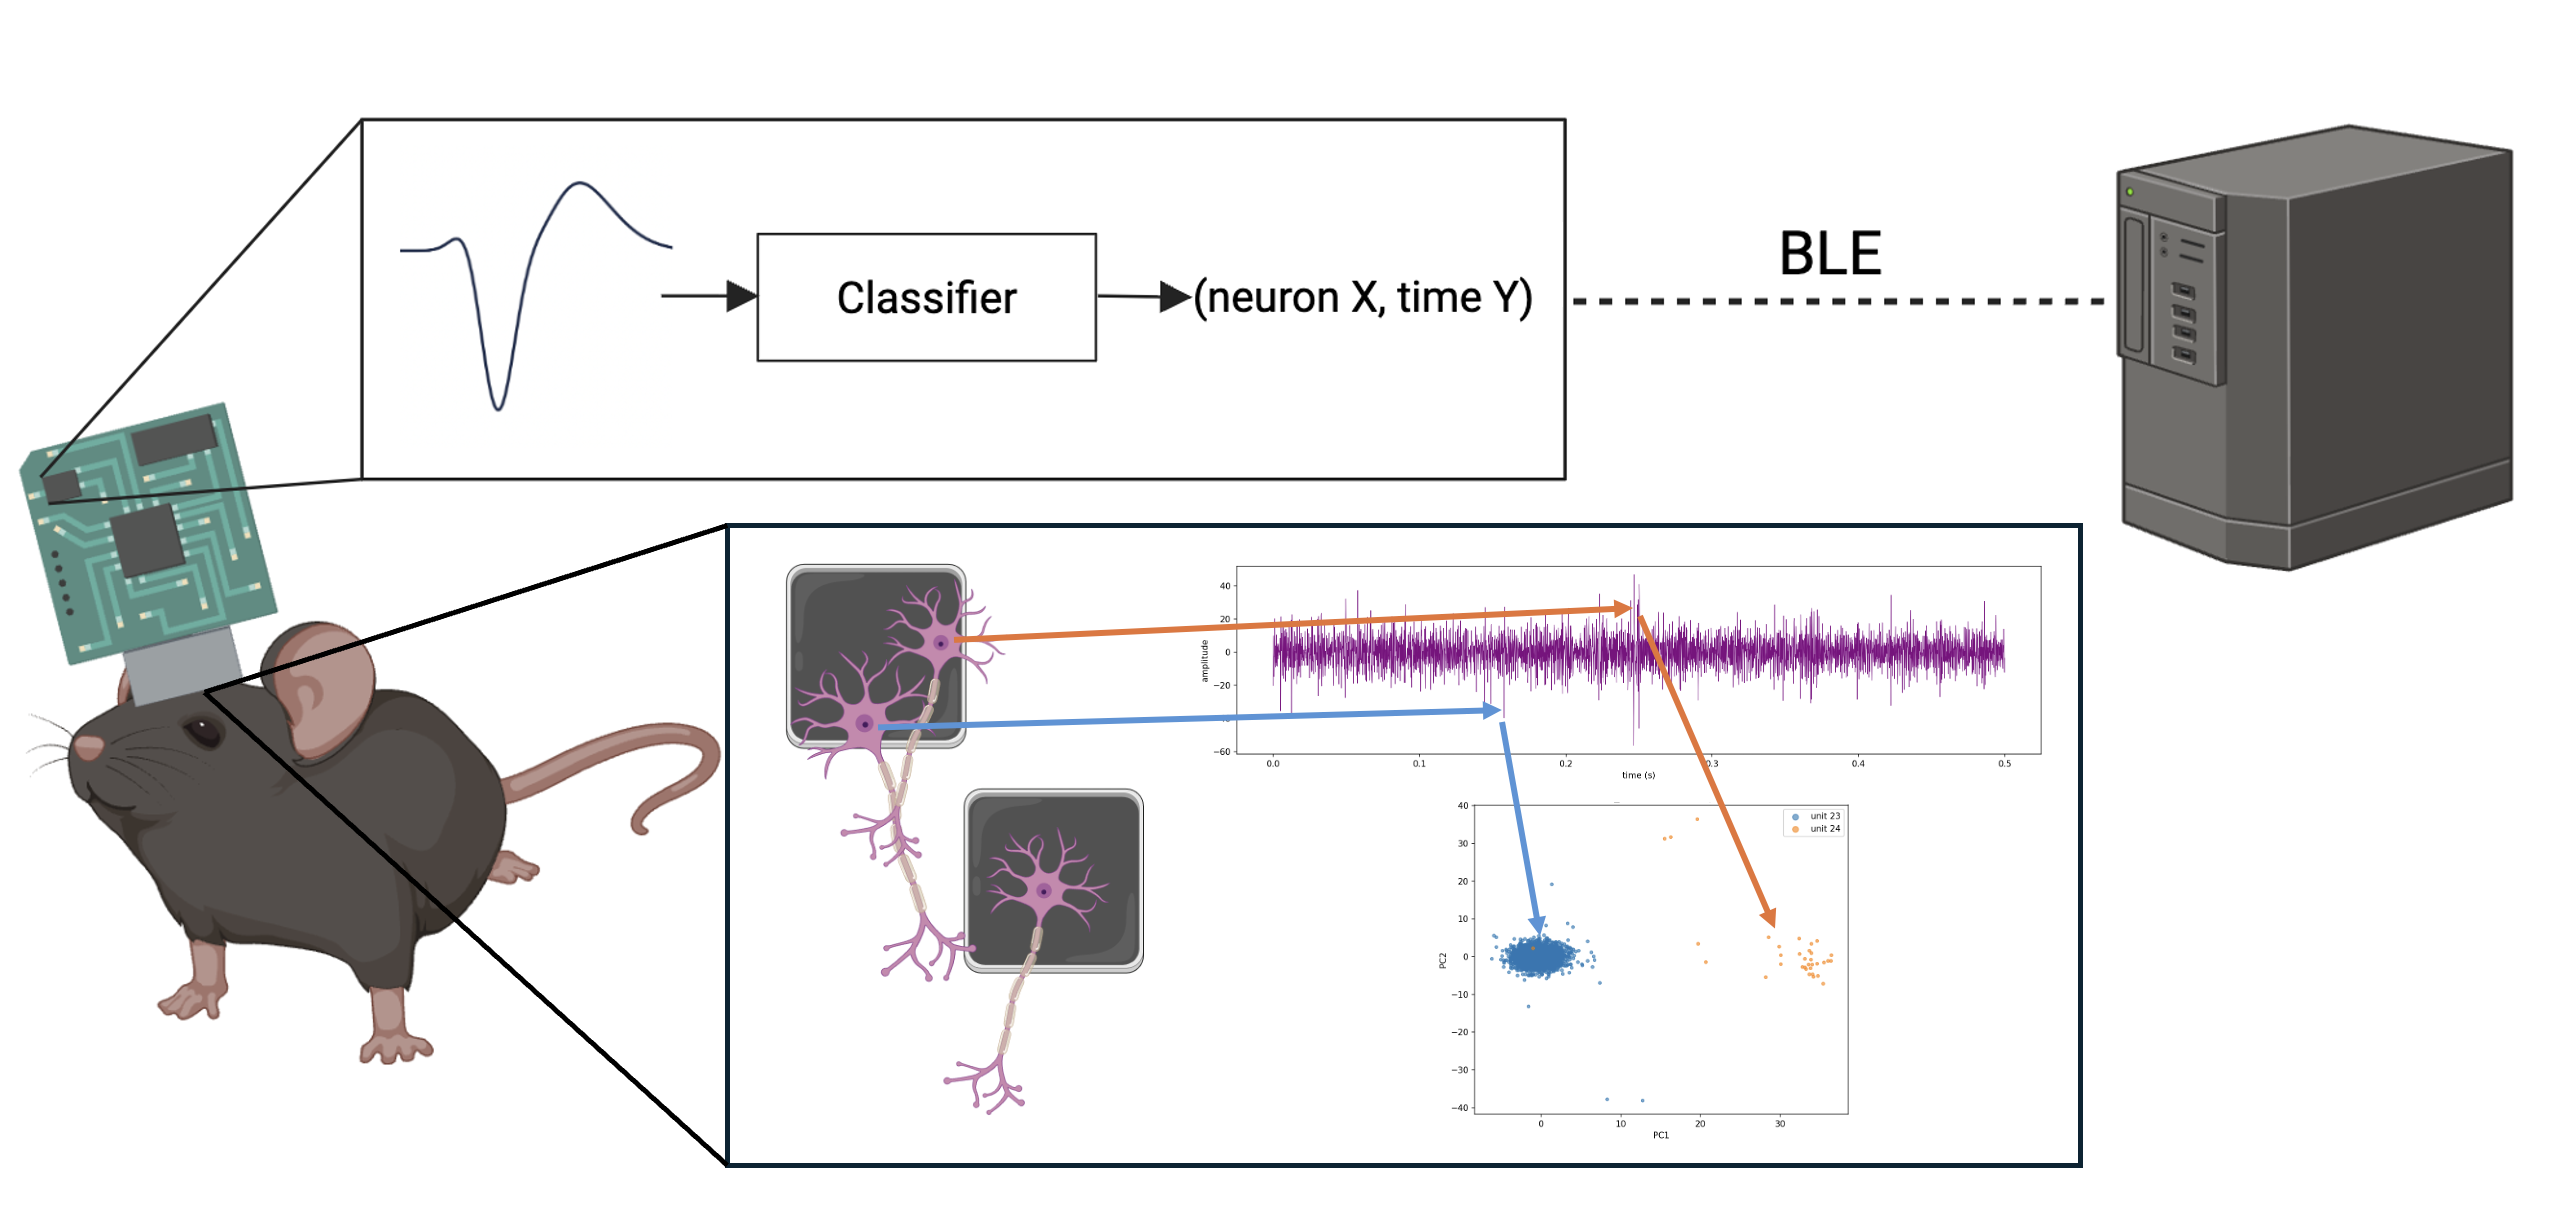
\includegraphics[width=\textwidth]{figures/figure1.png}
\caption{System overview. A head-mounted device classifies each detected extracellular
spike to its neuron of origin on-device and transmits only the resulting unit identity and
timestamp over Bluetooth Low Energy (BLE).}
\label{fig:overview}
\end{figure}

\vspace*{\fill}

\clearpage

% ======= 1. Problem Identification ======= %
\section{Problem Identification}

% ======= 1.1 Background and Motivation ======= %
\subsection{Background and Motivation}
Whether the substance of thought is reducible to physical processes remains an open
question. Nevertheless, evidence undisputedly suggests that the organized interplay between
neurons in the central nervous system gives rise to human sensory and cognitive
capacity~[1]. The first recording of what is now known as an action potential or
spike---the voltage across an electrically excitable cell's membrane as a function of
time---was published in 1868 by Julius Bernstein~[2]. Derived from frog tissue using a
differential rheotome, an apparatus he invented, Bernstein's measurement provided pivotal
evidence for theories regarding neural dynamics propounded by physicists and physiologists
preceding him~[2]. The interplay between neurons can, in turn, be studied by measuring the
action potentials of individual neurons within and across anatomically defined brain
regions~[3].

A desire to measure action potentials at increased scales has motivated the development of
high-density silicon recording probes. The Neuropixels 1.0 probe, introduced in 2017, is an
intracranial high-density probe for extracellular electrophysiology recordings in rodents
and is equipped with 384 channels for simultaneous recording~[3]. Its successor, the Neuropixels
2.0, was presented in 2021 and extends recording capacity to as many as 5120
channels~[4]. Such systems have enabled groundbreaking discoveries in systems neuroscience,
and the Neuropixels 3.0 is currently being developed~[5, 6]. Higher channel counts,
however, impose a proportionally higher bandwidth requirement whose improvement does not match
that of microfabrication.

The industry-standard analog front end for sampling raw extracellular voltage uses a 16-bit
analog-to-digital converter (ADC) typically configured with a 30~kHz sampling rate for roll-off
margin when recording 6kHz signals~[7,8]. At these settings, a full Neuropixels 2.0 quad-base recording produces a data rate of
$\sim$2.46~Gbps~[A1]. Bluetooth Low Energy 6.0 (BLE) is a state-of-the-art consumer
wireless communication protocol with a power budget suitable for an implantable
device~[9, 10]. In contrast to the data rate generated by state-of-the-art recording
probes, BLE has a theoretical maximum data rate of 2~Mbps~[9], just $\sim$0.08\% of the raw
data rate generated by a Neuropixels 2.0 quad-base recording~[A2]. Fortunately, many
questions in neuroscientific inquiry require only neural spike signatures, constituting a
small fraction of the continuous raw signal, enabling the compression design this proposal
suggests.~[11, 12].

% ======= 1.2 Stakeholders, Client, and End Used of the Solution ======= %
\subsection{Stakeholders, Client, and End User of the Solution}
Several groups have a stake in the project (Figure~\ref{fig:stakeholders}). The animals
that carry the device benefit most directly, because a wireless headstage frees them from
the recording cable and the stress it causes. Neuroscience as a field, and the agencies
that fund it, gain because recording more channels wirelessly allows experiments that are
impractical today. Preclinical drug research has an interest too, since studies of the
central nervous system often depend on recordings from animals that move freely.

The client is the neuroscience laboratory that would buy the device and use it in its own
work. These range from single academic groups to shared institutional facilities. Because
the design uses off-the-shelf parts, a lab can adopt it without building custom hardware.

The end users are systems neuroscientists. They study how neural activity relates to
behavior, which works best when the animal can move freely. Standard high-density recording
ties the animal to a cable that carries the raw data. This limits movement and rules out
experiments such as social interaction. A headstage that transmits wirelessly removes that
limit and lets researchers run a wider range of experiments.

\begin{figure}[H]
\centering
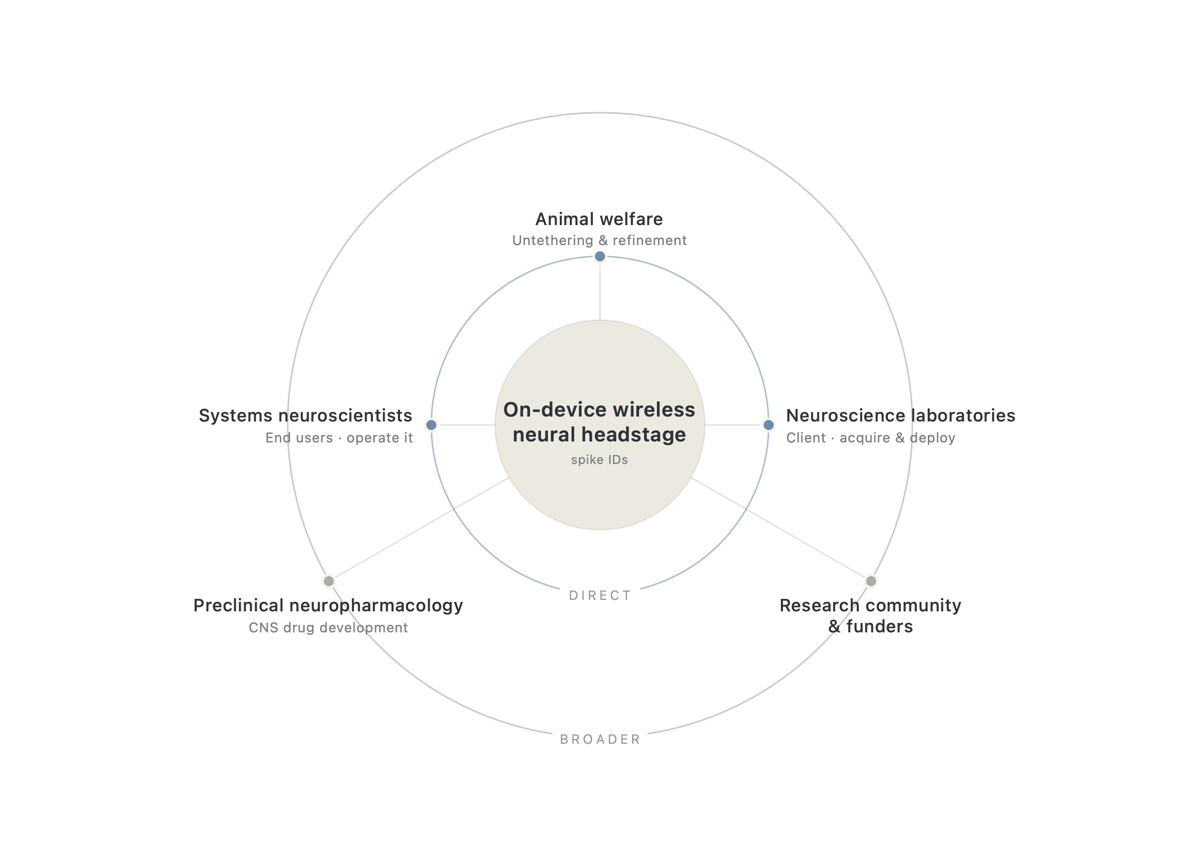
\includegraphics[width=0.75\textwidth]{figures/stakeholder_map.png}
\caption{Stakeholder map. Proximity to the center encodes directness of stake, from the
headstage at the core to its direct stakeholders (inner ring) and the broader stakeholders
(outer ring).}
\label{fig:stakeholders}
\end{figure}

% ======= 1.3 Problem Statement ======= %
\subsection{Problem Statement}
Since the onset of microfabrication techniques being applied for intracranial neural 
recording probe development, the rate of increase in channel count per recording probe 
has vastly outpaced the rate of increase in low-energy wireless bandwidth. Transmitting the 
entirety of continuous neural data for downstream processing was previously a reasonable design
when recording from a handful of metal electrodes. However, this wireless transmission design is not 
compatable with modern recording probes containing thousands of silicon recording channels. More precisely, 
the bandwidth of BLE is too low to transmit continuous neural data from more than four recording channels 
simultaneously, and data from thousands of channels is available. 


% ======= 2. Existing Solutions and Previous Work ======= %
\section{Existing Solutions and Previous Work}

% ======= 2.1 Existing Solutions ======= %
\subsection{Existing Solutions}
Two lines of work come close to this project without meeting: wireless headstages built
from commodity parts, and systems that classify spikes on the device. Each covers one half
of the problem. On the wireless side, headstages made from off-the-shelf parts already
record from freely-moving animals. The simplest stream the raw signal and do everything
offline; Tasneem et al.~[13] send raw data from a moving rat and detect and sort it
afterward. Gagnon-Turcotte et al.~[14] go a step further, pairing an Intan front end with a
Nordic radio to detect and compress spikes on the device, though the sorting into units
still happens at the receiver. In both, the link carries waveforms rather than neural
identities, so the bandwidth saving is modest.

On the other side, on-device classification has been taken furthest in custom silicon.
Fabricated spike-sorting chips reach 85--99\% classification accuracy on the device
itself~[15, 16, 17], which shows the algorithm fits a tight power and area budget. They
remain custom parts, though, tested only on replayed recordings and built with no radio, so
a neuroscience laboratory cannot simply obtain and use one.

The same on-device sorting also runs on commodity, programmable hardware. Luan et al.~[18]
perform real-time template matching on an Intan-plus-FPGA headstage in a freely-moving
primate, but log the result to an SD card. Wu et al.~[19] run an unsupervised sorter on an
FPGA at microsecond latency, again with no wireless link. These prove the classification
step is feasible off custom silicon, yet neither closes the wireless half.

The idea of splitting the work is not new either. Navajas and Quiroga~[20] showed in
simulation that templates can be built offline and each new spike matched on the device, so
that only the sorted identities travel over the link. What remains undone is to combine
these threads. No published system, to my knowledge, classifies single units on the device
and transmits their identities over a commodity Bluetooth Low Energy link, which is the
combination this project builds.

% ======= 2.2 Proposed Solution =======% 
\subsection{Proposed Solution}
This project proposes a recording head stage that detects spikes and classifies each to a
single unit on-device, transmitting only a unit identity and timestamp per spike
rather than the raw waveform. This design reduces the amount of data per spike by orders 
of magnitude, allowing far more channels to be streamed wirelessly than raw transmission 
permits while preserving the spatiotemporal spike information that neuroscientific analysis depends on.

% ======= 2.3 Previous Work ======= %
\subsection{Previous Work}
Only one part of the system has been built so far: a custom circuit board for testing the
signal path (Figure~\ref{fig:pcb}). It carries an Intan RHD2164 front end wired to an
nRF54LM20B over SPI. The board has been brought up and used to record a single channel from
end to end, with a known input passing through the Intan, across the SoC's Bluetooth Low
Energy link, and out to a laptop. This confirms the acquisition front end that the rest of
the system will build on.

\begin{figure}[H]
\centering
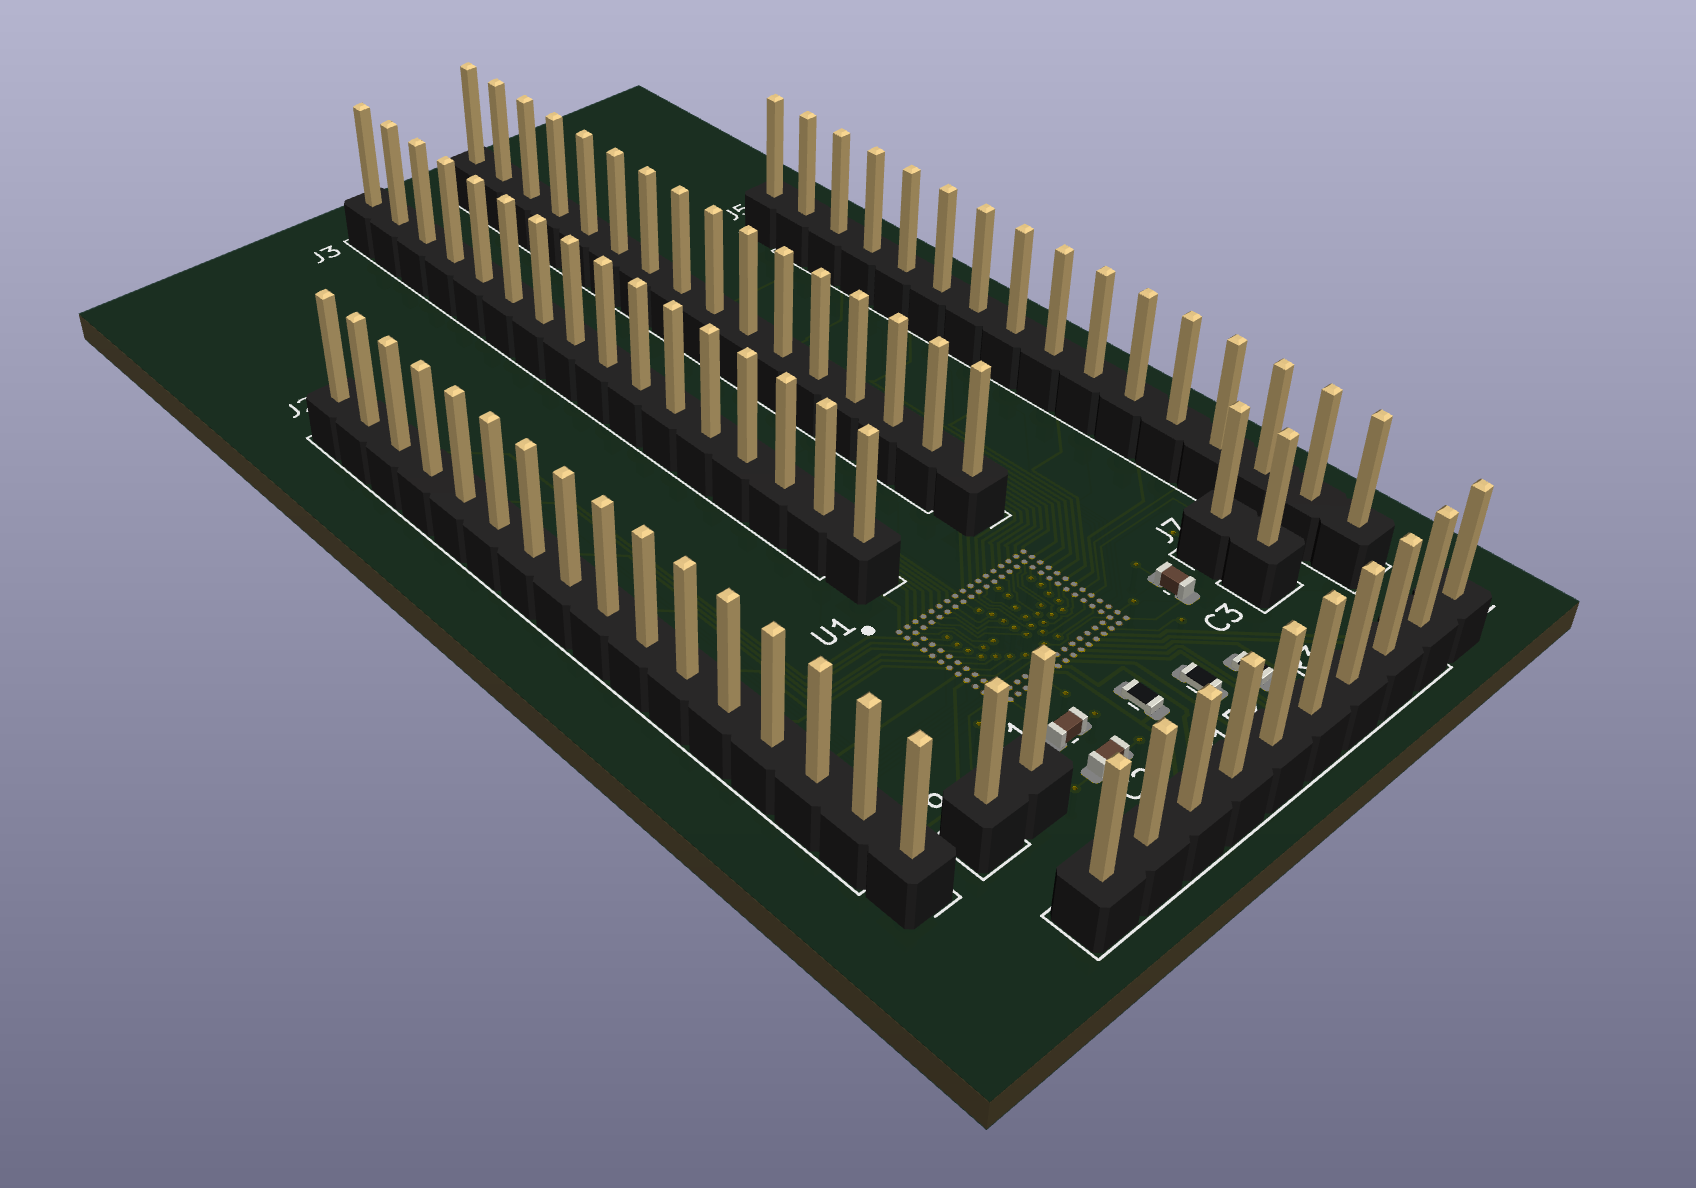
\includegraphics[width=0.6\textwidth]{figures/pcb.png}
\caption{Three-dimensional view of the custom signal-path test board, carrying the Intan
RHD2164 analog front end (BGA soldered on post fabrication).}
\label{fig:pcb}
\end{figure}

% ======= 3. Design Requirements and Technical Specifications ======= %
\section{Design Requirements and Technical Specifications}

% ======= 3.1 Description and Functional Requirements ======= % 
\subsection{Description and Functional Requirements}
This section decomposes the problem statement into the behaviors any valid solution must
exhibit (the functional requirements) and the qualitative conditions each behavior must
satisfy (the technical requirements). Each technical requirement is then made concrete as
a technical specification: a measurable parameter paired with a target value. These
requirements and specifications are stated independently of any particular design; the
design approaches that could realize them will be considered in-depth for checkpoint 1.

Compressing continuous neural data without fidelity loss of spatiotemporal spike
information requires isolating and preserving exactly the neural spike events at the
required resolution. Any solution to the problem statement must therefore
perform five operations: it must acquire extracellular voltage from multiple
recording channels, detect spike events within the acquired signal, log the
time at which each detected spike occurs, classify each detected spike and assign it
a unit identity, and transmit each unit identity coupled with its timestamp over a
wireless link. These five behaviors constitute the functional requirements of the system
summarized in Table~\ref{tab:funcreq}.

% ======= Table 1 ======= %
\begin{table}[H]
\centering
\caption{Functional requirements}
\label{tab:funcreq}
{\footnotesize
\setlength{\tabcolsep}{4pt}
\renewcommand{\arraystretch}{1.25}
\begin{tabularx}{\textwidth}{@{}l L@{}}
\toprule
Label & Functional requirement \\
\midrule
F1 & \emph{Acquire} extracellular voltage from multiple recording channels \\
F2 & \emph{Detect} spike events within the acquired signal \\
F3 & \emph{Log} the time at which each detected spike occurs \\
F4 & \emph{Classify} each detected spike and assign it a unit identity \\
F5 & \emph{Transmit} each unit identity coupled with its timestamp over a wireless link \\
\bottomrule
\end{tabularx}
}
\end{table}

% ======= 3.2 Technical Requirements and Specifications ======= %
\subsection{Technical Requirements and Specifications}
Each functional requirement imposes one or more technical requirements. 
Each requirement's specification draws its value from one of three sources: a first-principles calculation,
the prior-art literature, or preliminary testing conducted for this
project. The technical requirements are summarized in Table~\ref{tab:techreq}: T1 through T11
grouped by the functional requirement each serves, and T12 a system-level power constraint.
Justifications follow the table.

% ======= Table 2 ======= %
\begin{table}[H]
\centering
\caption{Technical requirements and specifications grouped by functional requirements}
\label{tab:techreq}
{\footnotesize
\setlength{\tabcolsep}{4pt}
\renewcommand{\arraystretch}{1.25}
\begin{tabularx}{\textwidth}{@{}l L L L@{}}
\toprule
Label & Requirement & Specification & Quantitative value \\
\midrule
\multicolumn{4}{@{}l}{\textbf{F1 --- Acquire}} \\
\addlinespace[2pt]
T1  & Acquire from more independent channels than a raw BLE link can carry & simultaneous channel count & $\geq 5$ (min); 32 (target) \\
T2  & Sample fast enough to capture the spike band without aliasing & per-channel sample rate & $\geq 12$~kS/s; 30~kS/s design point \\
T3  & Digitization keeps pace with every channel at once & aggregate conversion rate & $\geq$ channels $\times$ per-channel rate \\
T4  & Resolve spike amplitudes above the noise floor & ADC resolution; input-referred noise & 16-bit; $\leq 5~\mu$Vrms \\
T5  & Deliver the digitized stream to the processor without loss & ADC$\to$processor link throughput & $\geq$ channels $\times$ rate $\times$ bits \\
\midrule
\multicolumn{4}{@{}l}{\textbf{F2 --- Detect}} \\
\addlinespace[2pt]
T6  & Separate spikes from the local field potential & high-pass corner frequency & $\sim$300~Hz \\
T7  & Detect true spikes without over-triggering on noise & detection TPR / precision vs.\ Kilosort & TPR $\geq 90\%$; precision $\geq 90\%$ \\
\midrule
\multicolumn{4}{@{}l}{\textbf{F3 --- Log}} \\
\addlinespace[2pt]
T8  & Record when each detected spike occurs & timestamps per spike & one per detected spike \\
\midrule
\multicolumn{4}{@{}l}{\textbf{F4 --- Classify}} \\
\addlinespace[2pt]
T9  & Assign each detected spike a unit identity & unit label per spike & one of $K$ units \\
T10 & Classify better than chance & classification accuracy vs.\ Kilosort & $> 1/K$ (chance); aspirational 85--99\% \\
\midrule
\multicolumn{4}{@{}l}{\textbf{F5 --- Transmit}} \\
\addlinespace[2pt]
T11 & Transmit only the spike identity and its time, not the waveform & per-spike packet content & 5~B (1~B ID $+$ 4~B ts) \\
\midrule
\multicolumn{4}{@{}l}{\textbf{System-level}} \\
\addlinespace[2pt]
T12 & Run on a head-mounted battery for a useful session & average power draw & $\lesssim 100$~mW (target); $\geq 1$~h on a $<$1.5~g battery \\
\bottomrule
\end{tabularx}
}
\end{table}

% ======= Jusification of Technical Requirements and Specifications ======= %
\subsection{Justification of Technical Requirements and Specifications}
\textbf{Acquisition (F1).} Recording from at least five channels (T1) is the minimum that
beats the four-channel raw-BLE ceiling. Extracellular spikes occupy 300~Hz--6~kHz~[22], so
Nyquist sets a $\geq$12~kS/s per-channel floor~[A3]; the field-standard 30~kS/s~[7, 8] adds
oversampling margin (T2). The digitizer must convert every channel each sampling cycle (T3),
and the ADC-to-processor link must carry the resulting stream (T5), within the 8--32~Mbps
span of commodity BLE-SoC serial interfaces~[23]. A 16-bit converter with input-referred
noise under $\sim$5~$\mu$Vrms~[21] resolves the tens-to-hundreds-of-microvolt spikes clear of
the noise floor (T4).

\textbf{Detection (F2).} A high-pass corner near 300~Hz separates spikes from the sub-300~Hz
local field potential~[22] (T6). Detection is scored against Kilosort~[24]: since on-chip and
commodity detectors report 97--100\%~[14, 15, 16], a floor of 90\% sensitivity and 90\%
precision, matched within $\pm$1~ms, is conservative yet meaningful (T7).

\textbf{Timekeeping (F3).} Preserving spatiotemporal information requires one timestamp per
detected spike, referenced to the acquisition clock (T8).

\textbf{Classification (F4).} Each spike is assigned to one of $K$ units (T9). On-device
accuracy need only beat chance ($1/K$) against Kilosort labels~[24] to prove the pipeline
classifies rather than guesses; comparable on-chip sorters reach 85--99\%~[15, 16, 17], the
aspirational reference (T10).

\textbf{Transmission (F5).} Transmitting only a one-byte unit identity and a four-byte
timestamp per spike, five bytes, replaces the $\sim$80~bytes of a raw 40-sample snippet~[A4],
achieving the compression the solution depends on (T11).

\textbf{System-level (T12).} A head stage on a freely-moving animal must run on a small
onboard battery, not wall power or a data tether, so its power draw fixes the battery mass
and the length of a recording session. Transmitting only spike identities rather than raw
waveforms cuts the radio's airtime, so the compression that saves bandwidth also saves
transmission energy; both are quantified in the measurement plan.

% ======= 4. Plan for Measuring Technical Specifications ======= %
\section{Plan for Measuring Technical Specifications}

Every specification is verified on replayed or synthetic neural signals rather than live
animals, consistent with the scope of this project. The central instrument is a ground-truth
comparison. The same signal that reaches the nRF54 is split and fed in parallel to a tethered
reference recorder, so the two systems see an identical input. The reference recording is
sorted offline with Kilosort~4.0 to produce ground-truth spike times and unit labels, and the
on-device output is aligned to it through a shared synchronization marker and matched within a
$\pm$1~ms window. When the source is a synthetic recording built from a known file, its labels
serve as the ground truth directly. This split-signal setup is what makes detection (T7) and
classification (T10) measurable against truth rather than against the device's own output, and
it is the same architecture a later live-animal study would reuse.

Because the head stage rides a freely-moving animal, it must run on a small onboard battery; a
wall supply or a data tether would defeat the wireless purpose of the project. Power draw, and
the radio's share of it in particular, therefore sets the battery mass and the length of a
recording session. Power is measured as supply current times voltage under sustained
operation, with the transmission contribution isolated using a current profiler triggered on
the radio's activity, then converted into battery life for a candidate cell. Transmitting only
spike identities rather than raw waveforms cuts the radio's airtime by orders of magnitude, so
the same on-device classification that saves bandwidth is expected to save transmission energy;
measuring power with and without on-device classification quantifies that saving (T12).

The remaining specifications are characterized at the bench. Acquisition (T1--T5) uses a
function or arbitrary-waveform generator as the signal source, a logic analyzer on the SPI
bus, and firmware counters: channel count is read from the acquired stream, the per-channel
rate is confirmed by the spectrum of a known replayed tone and by the sampling-timer period,
aggregate throughput and link loss are counted as sustained conversions and dropped samples,
and front-end resolution and noise are measured from a shorted input and a known-amplitude
input. The filter corner and detection (T6--T7) come from a frequency sweep and from the
$\pm$1~ms match to Kilosort. Timekeeping, classification, and transmission (T8--T11) are read
from the received stream in software: one timestamp per event and its jitter against the sync
marker, a confusion matrix of unit assignments against Kilosort labels on held-out data, and
the five-byte content of each packet. Table~\ref{tab:measplan} pairs every specification with
its measurement method.

% ======= Table 3: specifications with measurement methods ======= %
\begin{table}[H]
\centering
\caption{Technical specifications paired with their measurement methods}
\label{tab:measplan}
{\footnotesize
\setlength{\tabcolsep}{4pt}
\renewcommand{\arraystretch}{1.25}
\begin{tabularx}{\textwidth}{@{}l L L L L@{}}
\toprule
Label & Requirement & Specification & Quantitative value & Measurement method \\
\midrule
\multicolumn{5}{@{}l}{\textbf{F1 --- Acquire}} \\
\addlinespace[2pt]
T1  & More channels than raw BLE carries & channel count & $\geq 5$; target 32 & count channels in the acquired stream \\
T2  & Sample fast enough for the band & per-channel sample rate & $\geq 12$~kS/s; 30~kS/s & FFT of a known replayed tone; timer period \\
T3  & Digitization keeps up & aggregate conversion rate & $\geq$ ch $\times$ rate & sustained and missed conversion counts \\
T4  & Resolve spikes above noise & resolution; noise & 16-bit; $\leq 5~\mu$Vrms & noise on a shorted input; SNR on a known input \\
T5  & Link carries the stream & ADC$\to$processor throughput & $\geq$ ch $\times$ rate $\times$ bits & sustained SPI rate; dropped-sample count \\
\midrule
\multicolumn{5}{@{}l}{\textbf{F2 --- Detect}} \\
\addlinespace[2pt]
T6  & Spikes separated from the LFP & high-pass corner & $\sim$300~Hz & filter response from a frequency sweep \\
T7  & Detect spikes reliably & TPR / precision vs.\ Kilosort & $\geq 90\%$ each & match to Kilosort truth, $\pm$1~ms window \\
\midrule
\multicolumn{5}{@{}l}{\textbf{F3 --- Log}} \\
\addlinespace[2pt]
T8  & A timestamp per detected spike & timestamp; jitter & one per spike & inspect stream; jitter vs.\ sync marker \\
\midrule
\multicolumn{5}{@{}l}{\textbf{F4 --- Classify}} \\
\addlinespace[2pt]
T9  & A unit identity per spike & unit label & one of $K$ & inspect output \\
T10 & Classify better than chance & accuracy vs.\ Kilosort & $> 1/K$; 85--99\% asp. & confusion matrix vs.\ Kilosort, held-out data \\
\midrule
\multicolumn{5}{@{}l}{\textbf{F5 --- Transmit}} \\
\addlinespace[2pt]
T11 & Packet carries identity and time & packet content & 5~B (1~B ID $+$ 4~B ts) & inspect received packets \\
\midrule
\multicolumn{5}{@{}l}{\textbf{System-level}} \\
\addlinespace[2pt]
T12 & Run on a head-mounted battery & power; radio share & $\lesssim 100$~mW; $\geq 1$~h on $<$1.5~g & current $\times$ voltage under load; profile radio; battery life \\
\bottomrule
\end{tabularx}
}
\end{table}


% ======= Appendix ======= %
\section*{Appendix}
\addcontentsline{toc}{section}{Appendix}

\noindent\textbf{[A1] Raw Neuropixels 2.0 data rate.} The aggregate raw rate is channel
count $\times$ per-channel sample rate $\times$ bit depth:
$5120 \times 30\text{~kS/s} \times 16\text{~bit} \approx 2.46$~Gbps.

\smallskip
\noindent\textbf{[A2] BLE share of the raw rate.} The BLE ceiling as a fraction of that raw
rate: $2\text{~Mbps} / 2.46\text{~Gbps} \approx 0.08\%$.

\smallskip
\noindent\textbf{[A3] Minimum spike-band sample rate.} By the Nyquist--Shannon sampling
theorem, faithfully capturing a band reaching $\sim$6~kHz requires
$f_s \geq 2 \times 6\text{~kHz} = 12$~kS/s.

\smallskip
\noindent\textbf{[A4] Raw snippet size.} A 40-sample spike snippet at 16-bit resolution is
$40 \times 16\text{~bit} = 640\text{~bit} = 80$~bytes, against the five-byte
identity-plus-timestamp packet of T11.

% ======= References ======= %
\phantomsection
\addcontentsline{toc}{section}{References}
\begin{thebibliography}{24}

\bibitem{ref1} E. R. Kandel, J. D. Koester, S. H. Mack, and S. A. Siegelbaum, \emph{Principles of Neural Science}, 6th ed. New York, NY, USA: McGraw-Hill, 2021.

\bibitem{ref2} E.-A. Seyfarth, ``Julius Bernstein (1839--1917): Pioneer neurobiologist and biophysicist,'' \emph{Biol. Cybern.}, vol. 94, no. 1, pp. 2--8, Jan. 2006.

\bibitem{ref3} J. J. Jun \emph{et al.}, ``Fully integrated silicon probes for high-density recording of neural activity,'' \emph{Nature}, vol. 551, no. 7679, pp. 232--236, Nov. 2017.

\bibitem{ref4} N. A. Steinmetz \emph{et al.}, ``Neuropixels 2.0: A miniaturized high-density probe for stable, long-term brain recordings,'' \emph{Science}, vol. 372, no. 6539, Art. no. eabf4588, Apr. 2021.

\bibitem{ref5} N. A. Steinmetz, P. Zatka-Haas, M. Carandini, and K. D. Harris, ``Distributed coding of choice, action and engagement across the mouse brain,'' \emph{Nature}, vol. 576, no. 7786, pp. 266--273, Dec. 2019.

\bibitem{ref6} IMEC and the Neuropixels Consortium, ``Neuropixels: Next-generation high-density neural probes,'' Leuven, Belgium, 2024. [Online]. Available: https://www.neuropixels.org

\bibitem{ref7} Intan Technologies, ``RHD2000-series digital electrophysiology interface chips (RHD2216/RHD2132),'' Datasheet, Los Angeles, CA, USA, 2021.

\bibitem{ref8} Intan Technologies, ``RHD2164 64-channel digital electrophysiology interface chip,'' Datasheet, Los Angeles, CA, USA, 2021.

\bibitem{ref9} Bluetooth Special Interest Group, ``Bluetooth core specification, version 6.0,'' Kirkland, WA, USA, 2024.

\bibitem{ref10} J. Tosi, F. Taffoni, M. Santacatterina, R. Sannino, and D. Formica, ``Performance evaluation of Bluetooth Low Energy: A systematic review,'' \emph{Sensors}, vol. 17, no. 12, Art. no. 2898, Dec. 2017.

\bibitem{ref11} H. G. Rey, C. Pedreira, and R. Quian Quiroga, ``Past, present and future of spike sorting techniques,'' \emph{Brain Res. Bull.}, vol. 119, pp. 106--117, Oct. 2015.

\bibitem{ref12} M. S. Lewicki, ``A review of methods for spike sorting: The detection and classification of neural action potentials,'' \emph{Network: Comput. Neural Syst.}, vol. 9, no. 4, pp. R53--R78, Nov. 1998.

\bibitem{ref13} N. Tasneem \emph{et al.}, ``A duty-cycled wireless optogenetic headstage for freely-moving rodents,'' \emph{IEEE Sensors J.}, vol. 23, no. 21, Nov. 2023.

\bibitem{ref14} G. Gagnon-Turcotte, Y. LeChasseur, C. Bories, Y. Messaddeq, Y. De Koninck, and B. Gosselin, ``A wireless optogenetic headstage with multichannel electrophysiological recording and in-situ spike detection and compression,'' \emph{IEEE Trans. Biomed. Circuits Syst.}, vol. 11, no. 1, pp. 129--141, Feb. 2017.

\bibitem{ref15} Z. Chen \emph{et al.}, ``A 128-channel spike-sorting SoC with level-crossing digitization and spatiotemporal feature extraction,'' \emph{IEEE Trans. Biomed. Circuits Syst.}, 2026.

\bibitem{ref16} Z. Jiang \emph{et al.}, ``A 1024-channel 583\,nW/channel spike-sorting SoC for high-density neural recording,'' \emph{IEEE Trans. Circuits Syst. I}, vol. 73, no. 8, 2026.

\bibitem{ref17} R. Lukito \emph{et al.}, ``A spike-sorting SoC with analog computing-in-memory autoencoder feature extraction,'' \emph{IEEE J. Solid-State Circuits}, vol. 61, no. 4, 2026.

\bibitem{ref18} S. Luan \emph{et al.}, ``Compact standalone platform for neural recording with real-time spike sorting and data logging,'' \emph{J. Neural Eng.}, vol. 15, no. 4, Art. no. 046014, 2018.

\bibitem{ref19} Z. Wu \emph{et al.}, ``A real-time unsupervised OSort spike-sorting processor implemented on FPGA,'' \emph{J. Neural Eng.}, vol. 20, no. 6, Art. no. 066015, 2023.

\bibitem{ref20} J. Navajas, D. Y. Barsakcioglu, A. Eftekhar, A. Jackson, T. G. Constandinou, and R. Quian Quiroga, ``Minimum requirements for accurate and efficient real-time on-chip spike sorting,'' \emph{J. Neurosci. Methods}, vol. 230, pp. 51--64, Jun. 2014.

\bibitem{ref21} R. R. Harrison, ``The design of integrated circuits to observe brain activity,'' \emph{Proc. IEEE}, vol. 96, no. 7, pp. 1203--1216, Jul. 2008.

\bibitem{ref22} G. Buzs\'aki, C. A. Anastassiou, and C. Koch, ``The origin of extracellular fields and currents---EEG, ECoG, LFP and spikes,'' \emph{Nat. Rev. Neurosci.}, vol. 13, no. 6, pp. 407--420, Jun. 2012.

\bibitem{ref23} Nordic Semiconductor, ``nRF54LM20B objective product specification,'' Trondheim, Norway, 2024.

\bibitem{ref24} M. Pachitariu, S. Sridhar, J. Pennington, and C. Stringer, ``Spike sorting with Kilosort4,'' \emph{Nat. Methods}, vol. 21, no. 5, pp. 914--921, May 2024.

\end{thebibliography}

\end{document}
